\documentclass{beamer}

\usepackage{amsmath}
\usepackage{amssymb}
\usepackage{graphicx}
\usepackage{subfigure}
\usepackage{multirow}
\usepackage{alphalph}
%\usepackage{animate}
% \usepackage{multimedia}
%\usepackage{caption}

%\usepackage{movie15}

\usepackage{appendixnumberbeamer}
\usetheme{Frankfurt}
%\xdefinecolor{maroon}{cmyk}{0.15,1.00,0.39,0.69}
%\xdefinecolor{maroon}{cmyk}{0.27,0.86,0.60,0.30}
%\xdefinecolor{maroon}{cmyk}{0.000,1.00,1.00,0.498}
\usecolortheme[RGB={80,0,0}]{structure}

% Shortcut commands
% My Shortcut Commands
\newcommand{\fig}[1]{Fig.~\ref{#1}}                      % figure
\newcommand{\tbl}[1]{Table~\ref{#1}}                     % table

\newcommand{\be}{\begin{equation*}}   % numbered equation
\newcommand{\ee}{\end{equation*}}

\newcommand{\benum}{\begin{equation}}   % numbered equation
\newcommand{\eenum}{\end{equation}}

\newcommand{\bea}{\begin{eqnarray*}}  % numbered equation array
\newcommand{\eea}{\end{eqnarray*}}

\newcommand{\beanum}{\begin{eqnarray}}  % numbered equation array
\newcommand{\eeanum}{\end{eqnarray}}

\newcommand{\eqt}[1]{Eq. (\ref{#1})}  % Reference to one equation
\newcommand{\eqts}[1]{Eqs. (\ref{#1})}  % Reference to multiple equations 

\newcommand{\vect}[1]{\ensuremath{ \vec{\mathbf #1}}}  % bold faced with vector arrow above
\newcommand{\B}[1]{\ensuremath{B_{#1} }}			% B with a sub scripted argument

\newcommand{\p}{\ensuremath{ \partial}}			% shortcut partial derivative symbol

\newcommand{\abs}[1]{\ensuremath{\left\lvert #1 \right\rvert}}  % absolute value of argument (variable bar size)
\newcommand{\norm}[1]{\ensuremath{\left\lVert #1 \right\rVert}}  % norm of argument, varaible size

\newcommand{\M}{\ensuremath{ \mathbf{M} }}
\newcommand{\R}{\ensuremath{ \mathbf{R} }}
\newcommand{\Lm}{\ensuremath{ \mathbf{L} }}
\newcommand{\D}{\ensuremath{ \mathbf{D} }}
\newcommand{\I}{\ensuremath{ \mathbf{I} }}

% Equation Punctuation
\newcommand{\pec}{\, ,}
\newcommand{\pep}{\, .}
\setbeamertemplate{footline}{
\leavevmode%
\hbox{\hspace*{-0.06cm}
\begin{beamercolorbox}[wd=.45\paperwidth,ht=2.25ex,dp=1ex,center]{author in head/foot}%
	\usebeamerfont{author in head/foot}Maginot %~~(\insertshortinstitute)
\end{beamercolorbox}%
\begin{beamercolorbox}[wd=.3\paperwidth,ht=2.25ex,dp=1ex,center]{section in head/foot}%
 Prelim Exam %\usebeamerfont{section in head/foot}\insertshorttitle
\end{beamercolorbox}%
\begin{beamercolorbox}[wd=.25\paperwidth,ht=2.25ex,dp=1ex,right]{section in head/foot}%
	\usebeamerfont{section in head/foot}March 31, 2014\hspace*{2em}
	\insertframenumber{} / \inserttotalframenumber\hspace*{2ex}
\end{beamercolorbox}}%
\vskip0pt%
}
\beamertemplatenavigationsymbolsempty
\beamertemplatetransparentcovered

\setbeamertemplate{bibliography item}[text]

\title{Preliminary Exam}
\author{Peter Maginot \\ Co-Chairs: Jim Morel and Jean Ragusa \\ Committee Members: Marvin Adams and Jean-Luc Guermond}
\institute{Texas A\&M University- Department of Nuclear Engineering}
\date{March 31, 2014 }


\newif\ifplacelogo % create a new conditional
\placelogotrue % set it to true
\logo{\ifplacelogo
\includegraphics[height=0.75cm]{CSGF_vert.eps}\fi}

\begin{document}
%---------------------------------------------------------------------------------------------
%\logo{
\includegraphics[height=0.75cm]{CSGF_vert.eps}}
\placelogofalse
\begin{frame}
\titlepage
\end{frame}

\begin{frame}
\begin{block}{Dissertation Goal}
\begin{center}
Methods for high-fidelity $ \color{black} S_N $ radiative transfer simulations
\end{center}
\end{block}
\begin{center}
\begin{Large}
\bf
Requirements to Achieve Goal
\end{Large}
\end{center}
\begin{enumerate}
\item Accurate Spatial Discretization
\begin{itemize}
\item Higher degree trial space DFEM
\item Must address robustness
\end{itemize}
\item Accurate Spatial Treatment of Opacities
\begin{itemize}
\item Cell-wise constant is a poor approximation for problems of interest
\end{itemize}
\item Efficient / Effective Acceleration
\begin{itemize}
\item Computationally efficient
\item Compatible with spatial discretization
\end{itemize}
\end{enumerate}

\end{frame}

\begin{frame}
\frametitle{Outline}
\tableofcontents[hideallsubsections]
%\begin{enumerate}
%\item Spatially Varying Cross Section Problems
%\item Low Order DSA for High Order DFEM Transport
%\item Strictly Non-Negative Bilinear Scheme for Unstrutured Quads
%\end{enumerate}
\end{frame}

\section[Lumping]{Lumping Techniques for High Order DFEM}
\subsection{1-D Slab DFEM Transport}
%
%\begin{frame}
%\frametitle{Starting from the bottom...}
%\benum
%\mu_d \frac{\p \psi_d}{\p x} + \sigma_t \psi_d(x) = \frac{\sigma_s(x)}{2} \phi(x) + q_d(x)
%\label{eq:ex_transport}
%\eenum
%\end{frame}

\placelogotrue

\begin{frame}
\frametitle{DFEM Discretization}
When we discretize the 1-D slab, mono-energetic, neutron transport equation with DGFEM, we get:
\be
\mu_d \mathbf{L}\vec{\psi}_d + \sigma_t \M \vec{\psi}_d = \frac{\sigma_s}{2} \M \vec{\phi} + \vec{q}_d + \psi_{in} \vec{f}
\ee
where we define the following (focusing only on $\mu_d > 0$):
\bea
\mathbf{L}_{ij} &=& \B{i}(1)\B{j}(1) - \int_{-1}^1{\frac{d \B{i}}{d s} \B{j}(s)~ds} \\
\mathbf{M}_{ij} &=& \frac{\Delta x}{2}\int_{-1}^1{ \B{i}(s) \B{j}(s)~ds} \\
\vec{f}_{i} &=& \B{i}(-1) \\
\vec{q}_{d,i} &=& \frac{\Delta x}{2} \int_{-1}^1{\B{i}(s) q_d(x)~ds} 
\eea
\end{frame}


\subsection{Matrix Lumping}
\begin{frame}
\frametitle{Matrix Lumping}

\begin{enumerate}
\item One method to improve the ``robustness'' 
\begin{itemize} 
\item solution positivity and resistance to oscillations
\end{itemize}
\item Lumping- makes diagonal mass matrices, does not guarantee change in robustness
\item Two ways to lump mass matrices
\begin{itemize}
\item Collapse an exactly integrated matrix's entries to the main diagonal
\item Use quadrature restricted to the DFEM interpolation points
\end{itemize} 
\item Both methods are equivalent for linear DFEM
\end{enumerate}

\end{frame}
%
%\begin{frame}
%\frametitle{Interpolation Points}
%Our DFEM basis functions, $\B{i}(s)$, are Lagrange interpolatory polynomials with interpolation points $s_j$.
%
%\end{itemize}
%
%\end{frame}

\begin{frame}
\frametitle{Self-Lumping Concept}
Since $\B{i}$ are interpolatory, restricting quadrature to the DFEM interpolation points creates a diagonal mass matrix  {\em automatically}
\begin{block}{Self-lumping (SL) $\mathbf{M}$}
\be
\mathbf{M}_{ij} = \left \{ \begin{array}{ll}  \frac{\Delta x }{2} w_i  & i=j \\ 0 & \text{otherwise} \end{array} \right.
\ee
\end{block}
\begin{itemize}
\item Typically, $s_j$ are chosen as equally-spaced points, and $\mathbf{L}$ and $\mathbf{M}_{\sigma}$ are integrated analytically
\item No requirement that $s_j$ be equally-spaced, could use more accurate quadrature as the interpolation points
\begin{itemize}
\item E.g. Gauss-Legendre (Gauss) or Lobatto-Gauss-Legendre (Lobatto)
\end{itemize}
\end{itemize}
\end{frame}

\subsection{New  Results}
\begin{frame}
\frametitle{Numerical Schemes}
\begin{block}{New to Dissertation}
\begin{small}
\begin{itemize} 
\item Self-lumping with higher degree trial spaces
\item Non equally-spaced interpolation points
\end{itemize}
\end{small}
\end{block}
\begin{itemize}
\item {\bf SL Gauss}: Gauss quadrature as interpolation points, quadrature restricted to interpolation points
\item {\bf SL Lobatto}: Lobatto quadrature as interpolation points, quadrature restricted to interpolation points
\item {\bf SL Newton-Cotes}: Equally-spaced points, quadrature (closed Newton-Cotes) restricted to interpolation points
\item {\bf TL} (Traditional Lumping): Equally-spaced points, analytic integration, then collapse to main diagonal
\item {\bf Exact DFEM}: Equally-spaced points, analytic integration
\end{itemize}
\end{frame}

\begin{frame}
\frametitle{Test Problem}
Source-free pure absorber, left incident flux, $\psi_{in,d}$, vacuum right BC.

Defining $h$:
\be
h = \frac{\sigma_t \Delta x}{\mu_d}
\ee
Analytic solution is
\be
\psi(x,\mu_d) = \psi_{in,d} \exp[-h]
\ee

\end{frame}

\begin{frame}
\frametitle{New Results (M\&C 2013)}
Positivity
\begin{itemize}
\item SL Gauss is strictly positive for even $P$
\item SL Lobatto and SL Newton-Cotes: strictly positive for odd $P$
\item TL not robust for $P>1$
\end{itemize}
Accuracy
\begin{itemize}
\item TL and SL Newton-Cotes converge $\norm{ \widetilde{\psi} - \psi }_{L^2} $ 2nd order for odd $P$, 3rd order for even $P$
\item SL Lobatto and SL Gauss converge $\norm{ \widetilde{\psi} - \psi }_{L^2} \propto P+1$
\end{itemize}
\end{frame}

\begin{frame}
\frametitle{Outflow Robustness}
\begin{columns}[c]
\column{0.5\textwidth}
\begin{figure}
\includegraphics[width=5.5cm]{P3_Outflow_AllMeth.eps}
\caption{$P=3$ Outflow as a function of $h$.}
\end{figure}
\column{0.5\textwidth}
\begin{figure}
\includegraphics[width=5.5cm]{P4_Outflow_AllMeth.eps}
\caption{$P=4$ Outflow as a function of $h$.}
\end{figure}
\end{columns}
\end{frame}

\begin{frame}
\frametitle{Order of Convergence}
Convergence of $\norm{ \widetilde{\psi} - \psi }_{L^2}$ as a function of $h$ 
\begin{columns}[c]
\column{0.5\textwidth}
\begin{figure}
\includegraphics[width=5.5cm]{Cubic_L2_err.eps}
\caption{$P=3$.}
\end{figure}
\column{0.5\textwidth}
\begin{figure}
\includegraphics[width=5.5cm]{Quartic_L2_err.eps}
\caption{$P=4$}
\end{figure}
\end{columns}
\end{frame}


\begin{frame}
\frametitle{New Results: Fixed Source Lumping (NS\&E)}
\begin{columns}[c]
\column{0.45\textwidth}
\begin{itemize}
\item Positivity of $\widetilde{\psi}(x)$ near inflow in source driven problem.
\item Vacuum, no incident flux
\item $\delta$ shaped source
\item Exact integration of RHS source moments is the most robust
\end{itemize}
 
\column{0.55\textwidth}
\begin{figure}
\includegraphics[width=5cm]{Final_Inflow_RHS_Comparison_Source_P3_MFP_0.eps}
\caption{Numerical solution near cell inflow.}
\end{figure}
\end{columns}
\end{frame}

\section[Cross Section]{Spatially Varying Cross Section}
\subsection{Background}

\begin{frame}
\frametitle{Motivation to Account for Cross Section Spatial Variation}
\begin{itemize}
\item Many problems of interest to the NE community have within cell spatially varying cross section/opacity
\begin{itemize}
\item Cross sections are functions of temperature, density, fuel burn-up, etc.
\item High fidelity simulations do not assume cell-wise constant values for these variables
\end{itemize}
\item Neutronics examples: fuel depletion problems, coupled reactor physics...
\item Radiative transfer: $\sigma = T^{-3}$
\end{itemize}
\end{frame}

\subsection{History}
\begin{frame}
\frametitle{History}
\begin{itemize}
\item Neutronics calculations almost exclusively approximate cross section as a cell-wise constant
\begin{itemize}
\item Some work has focused on assuming cross section is a linear function within cells
\item Focus of this historical work has been on reproducing fine mesh results with coarser zoning
\end{itemize}
\item Radiative transfer/radiative diffusion calculations (sometimes) account for within cell variation by using vertex based quadrature integration
\begin{itemize}
\item Idea introduced by Adams and Nowak circa 1997
\item Used by some (ex. Ober and Shadid ~2004)
\item Not by everyone
\end{itemize}
\end{itemize}
\end{frame}

\subsection{Extending Self-Lumping Framework}

\begin{frame}
\frametitle{SL Schemes for Spatially Varying Cross Section Problems}
\begin{itemize}
\item Trivial to extend quadrature integration to include spatial variation of cross section
\be
\mathbf{R}_{\sigma,ij}= \left \{ \begin{array}{ll}  \frac{\Delta x }{2}\sigma(s_i) w_i  & i=j \\ 0 & \text{otherwise} \end{array} \right.
\ee
where the DFEM equations that account for cross section spatial variation are:
\be
\mu_d \mathbf{L}\vec{\psi}_d + \R_{\sigma_t} \vec{\psi}_d = \frac{1}{2} \R_{\sigma_s} \vec{\phi} + \vec{q}_d + \psi_{in} \vec{f}
\ee
\item M\&C 2013 showed that exact mass matrix integration not required for full order accuracy schemes
\begin{itemize}
\item SL Lobatto does not exactly integrate $\mathbf{M}$ but has the same order of $L^2$ as SL Gauss
\end{itemize}
\end{itemize}
\end{frame}

\subsection{New Results (ANE 2014) }
\begin{frame}
\frametitle{Test Problem}
\begin{itemize}
\item Spatially varying cross section of the form:
\be
\sigma_t(x) = c_1 e^{c_2 x}
\ee
\item Incident flux, $\psi_{in,d}$ on the left, vacuum on the right, no sources.
\item Analytic Solution
\be
\psi(\mu_d,x) = \psi_{in,d}\exp\left[ \frac{c_1 }{\mu_d c_2 } \left(1- e^{c_2 x}  \right) \right] 
\ee
\end{itemize}
\end{frame}

\begin{frame}
\frametitle{Additional Numerical Schemes}
In addition to the self-lumping schemes, we will consider the following as well:
\begin{itemize}
\item {\bf CXS DFEM}: Equally-spaced interpolation points, analytic integration approximate cross section by cell average value
\item {\bf EXS DFEM}: Equally-spaced interpolation points, \\ (nearly) exact integration of cross section spatial dependence in the mass matrix
\end{itemize}
We will no longer consider the TL scheme.
\end{frame}

\begin{frame}
\frametitle{New Result: Robustness Is Not Guaranteed}
For an arbitrarily varying spatial cross section:
\begin{itemize}
\item Only linear SL Lobatto/SL Newton-Cotes yields strictly positive outflow:
\be
\widetilde{\psi}_{out} = \frac{2\mu_d^2 \psi_{in,d}}{2\mu_d^2 + \Delta x^2 \Sigma_{t,1} \Sigma_{t,2} + \Delta x \mu_d \Sigma_{t,1} + \Delta x \mu_d \Sigma_{t,2}}
\ee
%\item Higher order SL Lobatto and SL Newton-Cotes schemes are not strictly positive.
%\item SL Gauss is not strictly positive for any $P$
\item Angular flux outflow for all schemes that explicitly account for cross-section spatial variation is a function of cell optical thickness {\bf and} cross section spatial shape
\item Dependence on anything other than optical thickness is non-physical!
\end{itemize}
\end{frame}

\begin{frame}
\frametitle{Robustness-2}
Outflow for exponential $\sigma_t(s)$, constant optical thickness of 20 MFP, $\mu_d = 1$, $x\in[0,1~cm]$.
\begin{columns}[c]
\column{0.5\textwidth}
\begin{figure}
\includegraphics[width=5cm]{Exp_outflow_p2.eps}
\caption{Quadratic Trial Space.}
\end{figure}
\column{0.5\textwidth}
\begin{figure}
\includegraphics[width=5cm]{Exp_outflow_p3.eps}
\caption{Cubic Trial Space.}
\end{figure}
\end{columns}
\end{frame}

\begin{frame}
\frametitle{Convergence Results}
We examine the convergence of $E_{\psi}$ and $E_{\psi_{out}}$ for a pure absorber with
\be
\sigma_t(x) = 0.1~10^{2x}
\ee
and $x\in[0,1~cm]$.  We define the error quantities as:
\bea
E_{\psi} &=& \norm{ \widetilde{\psi}_d(x) - \psi(x,\mu_d)  }_{L^2} \\
E_{\psi_{out}} &=& \sqrt{\sum_{i=1}^{N_{cells}}{\Delta x_i\left(\widetilde{\psi}_{out,i} - \psi(x_{i+1/2})  \right)^2   }}  
\eea
\end{frame}

\begin{frame}
\frametitle{$L^2$ Convergence}
New Result: SL Lobatto and SL Gauss are accurate methods for spatially varying cross section problems
\begin{columns}[c]
\column{0.45\textwidth}
\begin{figure}
\includegraphics[width=5cm]{P3_VarXS_E_psi_L2.eps}
\caption{$P=3$ convergence plot.}
\end{figure}
\column{0.55\textwidth}
Summary of Convergence Orders
\begin{itemize}
\item SL Gauss: $\propto P+1$
\item SL Lobatto: $\propto P+1$, less accurate than SL Gauss
\item SL Newton-Cotes: 2 if odd $P$, 3 if even $P$
\item CXS DFEM: 2 regardless of $P$
\end{itemize}
\end{columns}
\end{frame}

\begin{frame}
\frametitle{$E_{\psi_{out}}$ Convergence}
\begin{columns}[c]
\column{0.45\textwidth}
\begin{figure}
\includegraphics[width=5cm]{P4_VarXS_E_psi_out.eps}
\caption{$P=4$ convergence plot.}
\end{figure}
\column{0.55\textwidth}
Summary of Convergence Orders
\begin{itemize}
\item SL Gauss: $2P+1$
\item SL Lobatto: $2P$
\item SL Newton-Cotes: $P+1$ for odd $P$,   $P+2$ for even $P$
\item CXS DFEM: $2P+1$
\end{itemize}
\end{columns}
\end{frame}

\section[Blading]{Interaction Rate}

\subsection{Interaction Rate}

\begin{frame}
\frametitle{Interaction Rate}
\begin{itemize}
\item Analytic interaction rate
\be
 IR(x) = \sigma_t(x) \psi(x,\mu_d)
\ee
\item CXS DFEM approximation
\be
\widetilde{IR}(x) = \hat{\sigma}_t \widetilde{\psi}(x)
\ee
\item SL schemes:  Only point-wise knowledge of $\sigma_t(x)$ in DFEM equations
\begin{itemize}
\item Integrals: evaluate $\widetilde{IR}(x)$ with quadrature restricted to interpolation points
\item Plotting purposes:
\be
\widetilde{IR}(x) = \sum_{j=1}^{P+1}{ \sigma_{t,j} \psi_j \B{j}(s) } 
\ee
\end{itemize}
\end{itemize}
\end{frame}

\begin{frame}
\frametitle{$L^2$ error of $\widetilde{IR}(x)$}

New Result: SL Lobatto and SL Gauss Accurately Approximate $\widetilde{IR}(x)$
\begin{columns}[c]
\column{0.55\textwidth}
\begin{figure}
\includegraphics[width = 5cm]{P3_VarXS_E_I_L2.eps}
\caption{Cubic DFEM}
\end{figure}
\column{0.45\textwidth}
Summary of Convergence Orders
\begin{itemize}
\item SL Gauss: $P+1$
\item SL Lobatto: $P+1$
\item SL Newton-Cotes: 2 for odd $P$, 3 for even $P$
\item CXS DFEM: 1, regardless of trial space degree
\end{itemize}
\end{columns}
\end{frame}

\begin{frame}
\frametitle{$E_{IR_A}$ Convergence}
\begin{columns}[c]
\column{0.45\textwidth}
\begin{figure}
\includegraphics[width = 5cm]{P4_VarXS_E_I_A.eps}
\caption{Quartic DFEM}
\end{figure}
\column{0.55\textwidth}
Summary of Convergence Orders
\begin{itemize}
\item SL Gauss: $2P+1$
\item SL Lobatto: $2P$
\item SL Newton-Cotes: $P+1$ for odd $P$, $P+2$ for even $P$
\item CXS DFEM: $2P+1$, regardless of trial space degree
\end{itemize}
\end{columns}
\end{frame}

\begin{frame}
\frametitle{CXS DFEM Accuracy Calculating $IR_A$}
\begin{itemize}
\item How can CXS DFEM converge $E_{IR_A}$ so accurately?
\item Local Conservation
\be
\text{Particles In} - \text{Particles Out} =  \text{Total Interactions} 
\ee
\item Particles In: Outflow from Previous Cell
\item Particles Out: Outflow from Current Cell
\item CXS DFEM converges angular flux outflow $\propto 2P+1$
\item $\therefore$ CXS DFEM accurately calculates
\be
\text{Total Interactions} =\Delta x \left( \widetilde{IR}_A \right)
\ee
\end{itemize}
\end{frame}


\subsection{Blading}
\begin{frame}
\frametitle{CXS DFEM Interaction Rate Profile}

\begin{block}{New to Dissertation}
Observation and explanation of blading phenomena
\end{block}
\begin{columns}[c]
\column{0.5\textwidth}
\begin{figure}
\includegraphics[width=5cm]{CXS_I_Blades.eps}
\caption{$\widetilde{IR}(x)$ profile.}
\end{figure}
\column{0.5\textwidth}
\begin{figure}
\includegraphics[width=5cm]{CXS_I_A_Profile.eps}
\caption{Interpolated $\widetilde{IR}_A$ profile.}
\end{figure}
\end{columns}

\end{frame}


\begin{frame}
\frametitle{Something Wrong with DFEM?}
No.  Consider the analytic solution to a problem that has the cell-wise average cross section.
\begin{columns}[c]
\column{0.5\textwidth}
\begin{figure}
\includegraphics[width=5cm]{Psi_Blades.eps}
\caption{Angular Flux.}
\end{figure}
\column{0.5\textwidth}
\begin{figure}
\includegraphics[width=5cm]{I_Blades.eps}
\caption{Interaction Rate.}
\end{figure}
\end{columns}

\end{frame}

\begin{frame}
\frametitle{Linear SL Lobatto Solution}
\begin{block}{New to Dissertation}
New: Self-lumping schemes do not exhibit blading
\end{block}
\begin{columns}[c]
\column{0.5\textwidth}
\begin{figure}
\includegraphics[width=5cm]{SLXS_Psi_Profile.eps}
\caption{Angular Flux.}
\end{figure}
\column{0.5\textwidth}
\begin{figure}
\includegraphics[width=5cm]{SLXS_I_Profile.eps}
\caption{Interaction Rate.}
\end{figure}
\end{columns}

\end{frame}

\section{Radiative Transfer }

\subsection{Radiative Transfer Equations with Material Spatial Dependence}

\begin{frame}
\frametitle{Grey, Spatially Analytic Radiative Transfer}
\begin{footnotesize}
\be
\frac{1}{c \Delta t}\left(I^{n+1} - I^n \right) + \mu \frac{\p }{\p x}I + \sigma_{t}^{n+1} I^{n+1} = \frac{\sigma_{s}^{n+1} }{4\pi}\phi^{n+1} + \sigma_{a} B(T^{n+1}) 
\ee
\be
\frac{C_v}{\Delta t}\left(T^{n+1} - T^n \right) = \sigma_a^{n+1} \left(\phi^{n+1}  - 4\pi B(T^{n+1})\right) 
\ee
\end{footnotesize}
\begin{small}
Linearizing the Plank function about an arbitrary temperature, $T^*$:
\end{small}
\begin{footnotesize}
\begin{multline}
\label{eq:rad}
\frac{1}{c \Delta t}\left(I^{n+1} - I^n \right) + \mu \frac{\p }{\p x}I^{n+1} + \sigma_{t}^{n+1} I^{n+1} = \\ \frac{\sigma_{s}^{n+1} }{4\pi}\phi^{n+1} + \sigma_{a}^{n+1} \left[ B(T^*) + \frac{\p B}{\p T} \bigg \lvert_{T=T^*} (T^{n+1} - T^*) \right]
\end{multline}
\begin{multline}
\label{eq:temp}
\frac{C_v^{n+1}}{\Delta t}\left(T^{n+1} - T^n \right) = \sigma_a^{n+1} \phi^{n+1}  \\ - 4\pi \sigma_a^{n+1} \left[ B(T^*) + \frac{\p B}{\p T} \bigg \lvert_{T=T^*} (T^{n+1} - T^*) \right]
\end{multline}
\end{footnotesize}
\end{frame}

\begin{frame}
\frametitle{Spatially Discretized Radiative Transfer}
\begin{small}
Drop $^{n+1}$ and discretize \eqt{eq:rad} and \eqt{eq:temp} with $P$ degree DFEM.
\end{small}
\begin{multline}
\label{eq:rad_disc}
\frac{1}{c \Delta t}\M\left(\vec{I} - \vec{I}^n \right) + \mu \Lm \vec{I} + \R_{\sigma_t} \vec{I} = \\ 
\frac{1}{4\pi}\R_{\sigma_s} \vec{\phi} + \R_{\sigma_a} \left[ \vec{B^*} + \D (\vec{T} - \vec{T^*}) \right] + \vec{f} I_{in}
\end{multline}
\benum
\label{eq:temp_disc}
\frac{1}{\Delta t}\R_{C_v} \left(\vec{T} - \vec{T}^n \right) = \R_{\sigma_a} \left\{ \vec{ \phi}  - 4\pi \left[ \vec{B^*} + \D (\vec{T} - \vec{T^*}) \right] \right \}
\eenum
\begin{small}
Define $(P+1) \times (P+1)$ diagonal matrix \D ~and $(P+1) \times 1$ vector $\vec{B^*}$:
\end{small}
\bea
\D_{ii} &=& \frac{\p B}{\p T }\bigg \lvert_{T = T^*_i}\\
\vec{B^*}_i &=& B(T^*_i)
\eea 
\end{frame}

\begin{frame}
\frametitle{Solving for $\vec{T}$}
Solve \eqt{eq:temp_disc} for $\vec{T}$, use in \eqt{eq:rad_disc} to eliminate $T^{n+1}$ dependence.
%\be
%\frac{1}{\Delta t}\R_{C_v} \vec{T} + 4\pi \R_{\sigma_a} \D \vec{T} = \frac{1}{\Delta t}\R_{C_v} \vec{T^n}  + \R_{\sigma_a} \left[ \vec{ \phi} - 4\pi \vec{B^*} + 4\pi \D \vec{T^*} \right] 
%\ee

\begin{multline*}
\left[ \I + 4\pi \Delta t \R_{C_v}^{-1} \R_{\sigma_a} \D  \right]\vec{T} = \vec{T^n}  +  \Delta t \R_{C_v}^{-1} \R_{\sigma_a}  \vec{ \phi}  \\ -
 4\pi \Delta t \R_{C_v}^{-1} \R_{\sigma_a}  \left[  \vec{B^*} - \D \vec{T^*} \right] 
\end{multline*}
Adding ``zero'' to both sides
\be
= + \I \left[\vec{T^*} - \vec{T^*} \right]
\ee
Get a Newton update for $\vec{T^{(n+1)}}$
\begin{multline}
\label{eq:t_iso}
\vec{T} = \vec{T^*} + \left[ \I + 4\pi \Delta t \R_{C_v}^{-1} \R_{\sigma_a} \D  \right]^{-1} \left[  (\vec{T^n}-\vec{T^*}) \right] +  \\
\left[ \I + 4\pi \Delta t \R_{C_v}^{-1} \R_{\sigma_a} \D  \right]^{-1}  \Delta t \R_{C_v}^{-1}\R_{\sigma_a} \left[ \vec{ \phi} - 4\pi \vec{B^*} \right] 
\end{multline}
\end{frame}

\begin{frame}
\frametitle{Forming the Radiation Equation}
\begin{enumerate}
\item \eqt{eq:t_iso} is inserted into the radiation equation, \eqt{eq:rad_disc}
\item The only unknown in this new equation is $\vec{I}^{n+1}$
\begin{itemize}
\item Opacities are evaluated at $\vec{T^*}$
\end{itemize}
\item \eqt{eq:t_iso} becomes a Newton iteration for $\vec{T^*}$
\item Cannot isolate $\vec{T}^{n+1}$ if $\frac{\p \sigma}{\p T}$ terms accounted for
\item No observed stability/convergence issues with updating $\sigma$ in a fixed-point style
\item New radiation equation (next slide) can be written in pseudo-fission format
\begin{itemize}
\item DFEM unknowns de-couple with SL schemes (diagonal \R)
\end{itemize}
\end{enumerate}
\end{frame}


\begin{frame}
\frametitle{Pseudo-Fission Form of Radiation Equation}
\benum
\mu \Lm \vec{I} +\R_{\sigma_{\tau}} \vec{I} = \frac{1}{4\pi}\R_{\sigma_s} \vec{\phi} + \frac{1}{4\pi}\bar{\bar{\nu}} \R_{\sigma_a}\vec{\phi} + \bar{\xi} + \vec{f} I_{in}
\label{eq:pseudo_fission}
\eenum
Where we have made the following definitions:
\bea
\R_{\sigma_{\tau} }&=& \frac{1}{c\Delta t}\M + \R_{\sigma_t} \\
\bar{\bar{\nu}} &=& 4\pi \R_{\sigma_a}\D  \left[ \I+ 4\pi \Delta t \R_{C_v}^{-1} \R_{\sigma_a} \D  \right]^{-1}  \Delta t \R_{C_v}^{-1} \\
\bar{\xi} &=& \R_{\sigma_a} \vec{B^*}  + \R_{\sigma_a}\D  \left[ \I+ 4\pi \Delta t \R_{C_v}^{-1} \R_{\sigma_a} \D  \right]^{-1}  \left[  \vec{T^n}-\vec{T^*} \right] \\
&\dots & -4\pi \R_{\sigma_a} \D \left[ \I+ 4\pi \Delta t \R_{C_v}^{-1} \R_{\sigma_a} \D  \right]^{-1} \Delta t \R_{C_v}^{-1}\R_{\sigma_a} \vec{B^*}  
\eea

\end{frame}
\placelogofalse
\begin{frame}
\frametitle{SL Lobatto Radiative Transfer Solution}
\begin{block}{New to Dissertation}
Observation of radiative transfer temperature blading, explanation of why, and a viable solution to the problem
\end{block}
\begin{columns}[c]
\column{0.5\textwidth}
\begin{figure}[!htp]
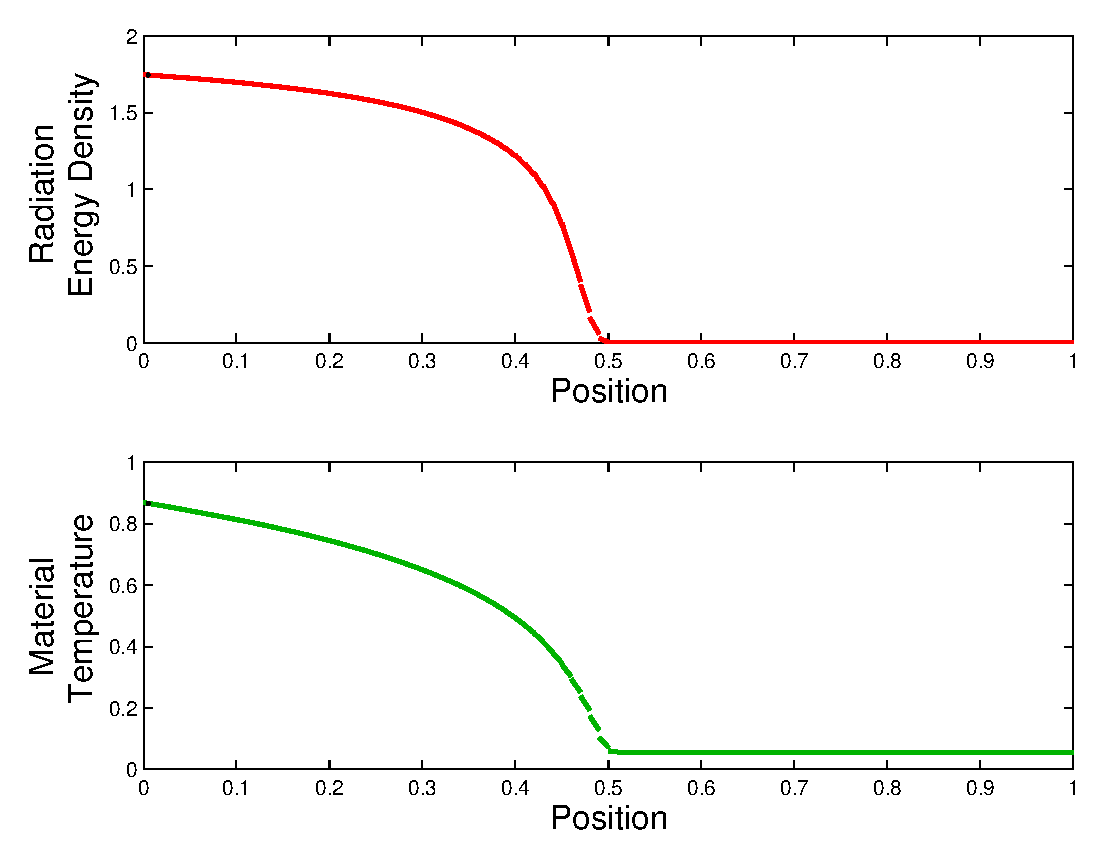
\includegraphics[width=5cm]{Proposal_ex_sol.eps}
\caption{Linear SL Lobatto solution to the Marshak wave problem.}
\end{figure}
\column{0.5\textwidth}
\begin{figure}[!htp]
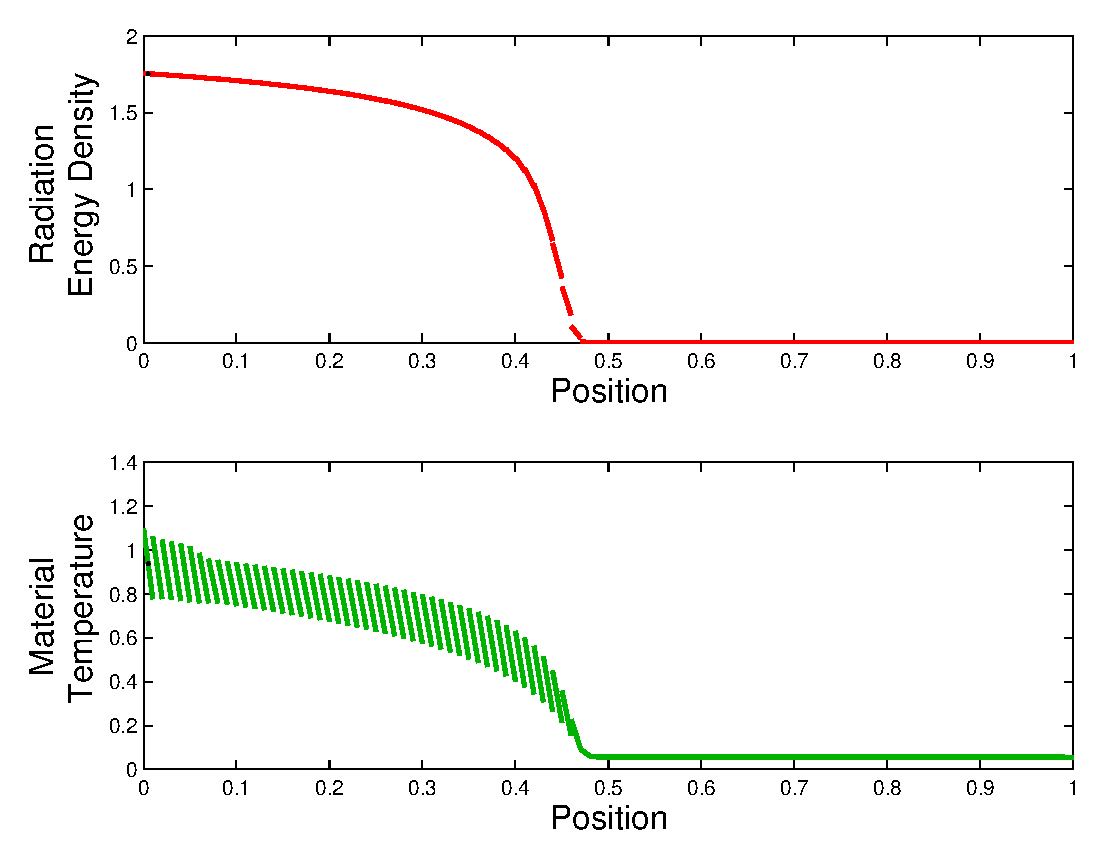
\includegraphics[width=5cm]{Proposal_blades.eps}
\caption{Linear, traditional lumping, constant cross section solution to the Marshak wave problem.}
\end{figure}
\end{columns}
\end{frame}

\section[MIP DSA]{Low Order MIP DSA for High Order DFEM Transport}
\subsection{MIP}
\begin{frame}
\frametitle{Third Known Use of MIP DSA!}
\begin{columns}[c]
\column{0.35\textwidth}
Neutronics Spectral Radius Test:
\begin{itemize}
\item Slab, $80~[cm]$ thick 
\item $\sigma_t = 10~[cm^{-1}]$
\item $c=0.9999$
\item $S_{16}$ quadrature
\item Random initial solution
\end{itemize}

\column{0.65\textwidth}
\begin{figure}
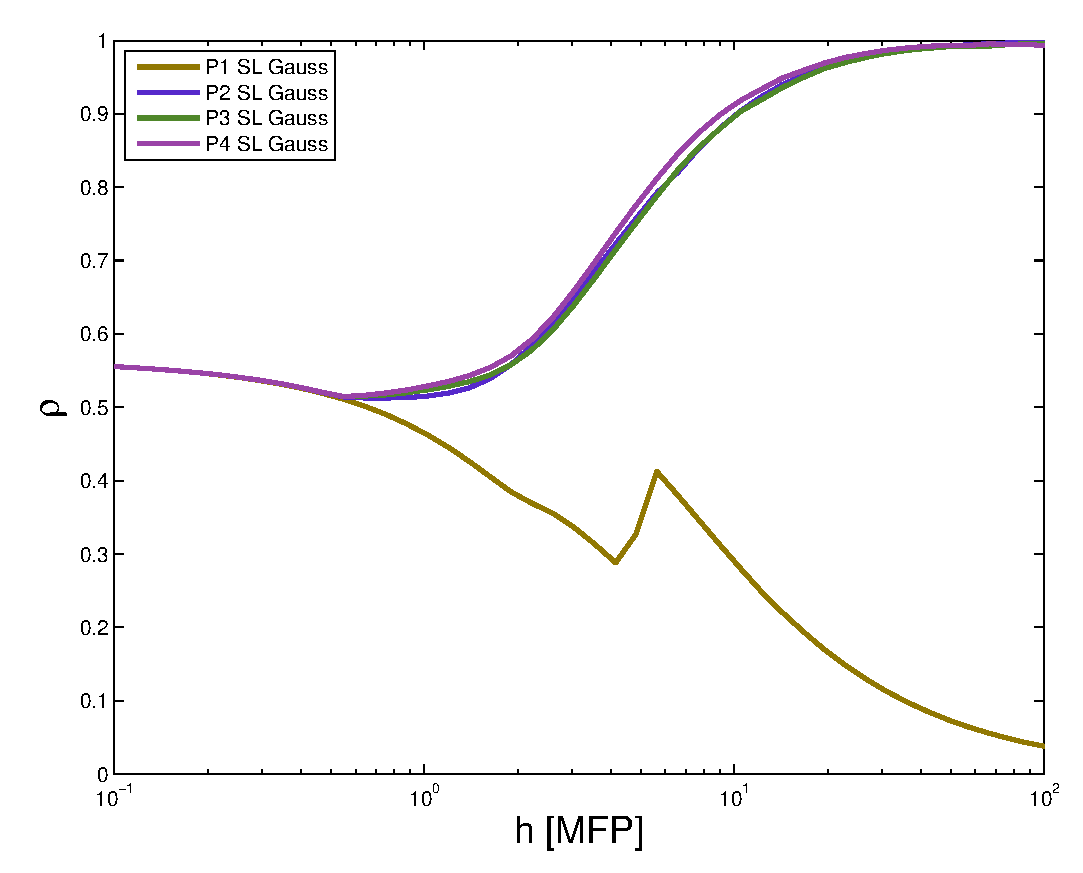
\includegraphics[width =7cm]{SL_Gauss_MIP_SPR.eps}
\caption{Numerical SPR for $P$ degree SL Gauss transport with $P=1$ SL Gauss MIP DSA}
\end{figure}
\end{columns}
\end{frame}

\begin{frame}
\frametitle{Krylov with Low Order MIP}
\begin{columns}[c]
\column{0.4\textwidth}
\begin{itemize}
\item $80~[cm]$ slab
\item $\sigma_t = 10~[cm^{-1}]$
\item $c=0.9999$
\item $S_{16}$ quadrature
\item Uniform, isotropic source, vacuum BC
\end{itemize}
\column{0.6\textwidth}
\begin{figure}
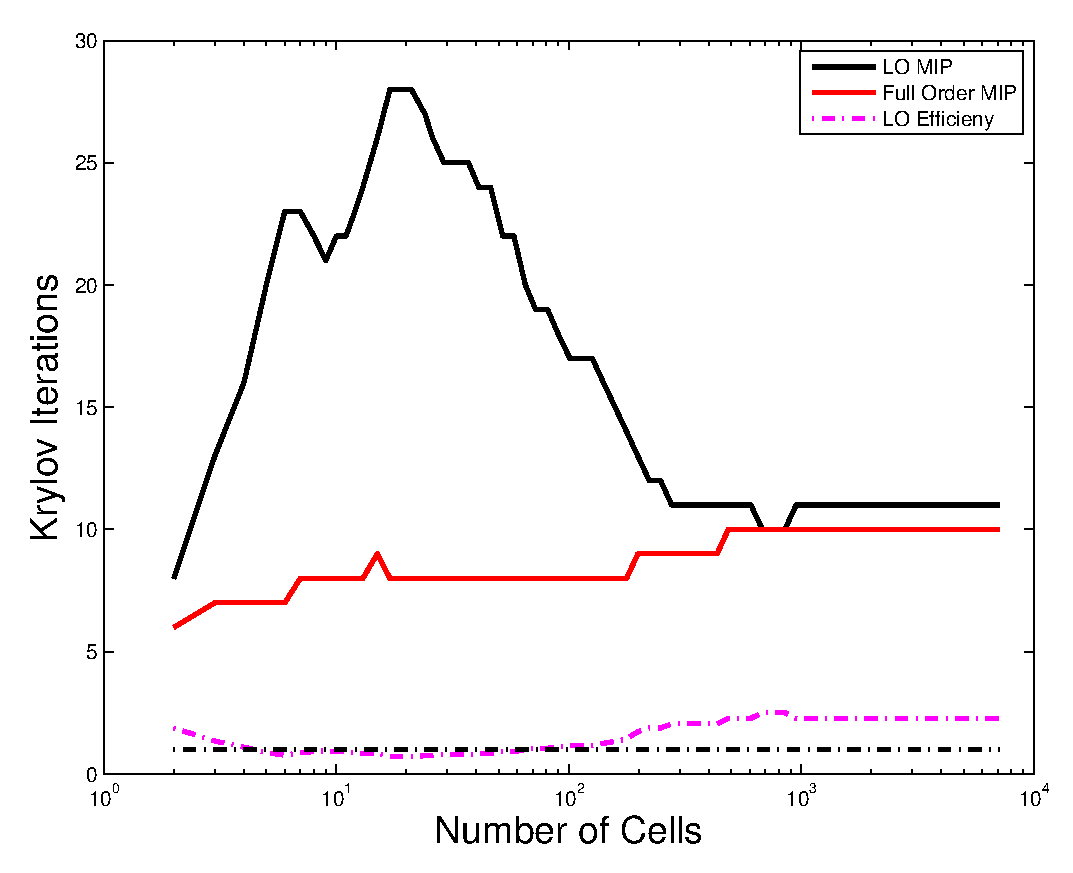
\includegraphics[width=7cm]{Krylov_Comp_p4_sl_Gauss.eps}
\caption{$P=4$ SL Gauss transport}
\end{figure}
\end{columns}
\end{frame}

\placelogotrue

\section{Future Work}
\subsection{C++ Code}
\begin{frame}
\frametitle{Work to Be Completed}
Slab, Multi-frequency $S_N$ Radiative Transfer Code
\begin{itemize}
\item C++
\item Arbitrary trial space degree
\item Lobatto, Gauss, and equally-spaced interpolation points
\item Arbitrary SDIRK time integration
\item Fixed-point and Krylov for solving within group scattering 
\item Fixed-point and Krylov for absorption/re-emission iteration
\item MIP DSA/LMFGA operators
\item Use PETSc / Trillinos for GMRES and inverting diffusion operators
\end{itemize} 
Complete non-negative, unstructured mesh bilinear DFEM implementation in PDT (98\% done)
\end{frame}

\begin{frame}
\frametitle{Questions?}
\end{frame}

%\appendix
%
%\begin{frame}
%\frametitle{Pseudo-fission Workout}
%\begin{multline*}
%\frac{1}{c \Delta t}\M\left(\vec{I} - \vec{I}^n \right) + \mu \Lm \vec{I} + \R_{\sigma_t} \vec{I} = 
%\frac{1}{4\pi}\R_{\sigma_s} \vec{\phi} + \vec{f} I_{in} + \R_{\sigma_a} \vec{B^*} + \\
%\R_{\sigma_a}\D \left[  \I + 4\pi \Delta t \R_{C_v}^{-1} \R_{\sigma_a} \D  \right]^{-1} \left[  (\vec{T^n}-\vec{T^*}) \right] +  \\
%\Delta t \R_{\sigma_a}\D  \left[ \I+ 4\pi \Delta t \R_{C_v}^{-1} \R_{\sigma_a} \D  \right]^{-1}   \R_{C_v}^{-1}\R_{\sigma_a} \left[ \vec{ \phi} - 4\pi \vec{B^*} \right] 
%\end{multline*}
%Group Terms
%\begin{multline*}
%\mu \Lm  \vec{I} + \R_{\sigma_{\tau}} = \frac{1}{4\pi}\R_{\sigma_s}\vec{\phi} + \Delta t \R_{\sigma_a}\D  \left[ \I+ 4\pi \Delta t \R_{C_v}^{-1} \R_{\sigma_a} \D  \right]^{-1}   \R_{C_v}^{-1}\R_{\sigma_a} \vec{ \phi} \\
%+ \R_{\sigma_a} \vec{B^*}  + \R_{\sigma_a}\D  \left[ \I+ 4\pi \Delta t \R_{C_v}^{-1} \R_{\sigma_a} \D  \right]^{-1}  \left[  \vec{T^n}-\vec{T^*} - 4\pi  \Delta t \R_{C_v}^{-1}\R_{\sigma_a} \vec{B^*}  \right] + \vec{f} I_{in}
%\end{multline*}
%\end{frame}
%
%\begin{frame}
%\frametitle{Fitting Pseudo-Fission to DSA Needs}
%DSA solves:
%\be
%-\nabla D_{DSA} \nabla \phi + \sigma_{a,DSA} \phi = q
%\ee
%With Fick's law, we define
%\be
%D_{DSA} = \frac{1}{3\sigma_{t,DSA}}
%\ee
%What are $\sigma_a$ and $\sigma_t$ from the pseudo-fission radiation equation?
%\end{frame}
%
%\begin{frame}
%\frametitle{Fitting Pseudo-Fission to DSA Needs-2}
%\eqt{eq:pseudo_fission} is a transport equation:
%\be
%\mu \Lm \psi + \sigma_t \psi = \frac{\sigma_s}{4\pi} \phi 
%\ee
%Therefore
%\be
%\sigma_{t,DSA} = \frac{1}{c\Delta t} + \sigma_t
%\ee
%and since $\sigma_a = \sigma_t - \sigma_s$
%\bea
%\sigma_{a,DSA} &=& \left( \frac{1}{c\Delta t} + \sigma_t \right) - \frac{4\pi \sigma_a \frac{\p B}{\p T}\bigg \lvert_{T^*}\Delta t  }{C_v + 4\pi \Delta t\sigma_a  \frac{\p B}{\p T}\bigg \lvert_{T^*}} \sigma_a \\
%\sigma_{a,DSA} &=& \left( \frac{1}{c\Delta t} + \sigma_t \right) - \frac{4\pi \sigma_a \frac{\p B}{\p T}\bigg \lvert_{T^*}}{ \frac{C_v}{\Delta t} + 4\pi \sigma_a  \frac{\p B}{\p T}\bigg \lvert_{T^*}} \sigma_a
%\eea
%
%\end{frame}


%%\section{Extra Graphs}
%\begin{frame}
%\frametitle{Robustness}
%Outflow for exponential $\sigma_t(s)$, constant optical thickness of 20 MFP, $\mu_d = 1$, $x\in[0,1~cm]$.
%\begin{figure}[!hbp]
%\subfigure[Linear]{
%\includegraphics[width=0.45\textwidth]{Exp_outflow_p1.eps}
%}
%\subfigure[Quadratic]{
%\includegraphics[width=0.45\textwidth]{Exp_outflow_p2.eps}
%}
%%\subfigure[Cubic]{
%%\includegraphics[width=0.4\textwidth]{Exp_outflow_p3.eps}
%%}
%%\subfigure[4-th Order]{
%%\includegraphics[width=0.4\textwidth]{Exp_outflow_p4.eps}
%%}
%\end{figure}
%\end{frame}
%
%\begin{frame}
%\frametitle{Robustness}
%Outflow for exponential $\sigma_t(s)$, constant optical thickness of 20 MFP, $\mu_d = 1$, $x\in[0,1~cm]$.
%\begin{figure}[!hbp]
%%\subfigure[Linear]{
%%\includegraphics[width=0.45\textwidth]{Exp_outflow_p1.eps}
%%}
%%\subfigure[Quadratic]{
%%\includegraphics[width=0.45\textwidth]{Exp_outflow_p2.eps}
%%}
%\subfigure[Cubic]{
%\includegraphics[width=0.45\textwidth]{Exp_outflow_p3.eps}
%}
%\subfigure[Quartic]{
%\includegraphics[width=0.45\textwidth]{Exp_outflow_p4.eps}
%}
%\end{figure}
%\end{frame}
%
%\begin{frame}
%\frametitle{$E_{\psi}$ Convergence}
%\begin{figure}
%\subfigure[Linear]{
%\includegraphics[width=5cm]{P1_VarXS_E_psi_L2.eps}
%}
%\subfigure[Quadratic]{
%\includegraphics[width=5cm]{P2_VarXS_E_psi_L2.eps}
%}
%\end{figure}
%\end{frame}
%
%\begin{frame}
%\frametitle{$E_{\psi}$ Convergence}
%\begin{figure}
%\subfigure[Cubic]{
%\includegraphics[width=5cm]{P3_VarXS_E_psi_L2.eps}
%}
%\subfigure[Quartic]{
%\includegraphics[width=5cm]{P4_VarXS_E_psi_L2.eps}
%}
%\end{figure}
%\end{frame}
%
%\begin{frame}
%\frametitle{$E_{\psi_A}$ Convergence}
%\begin{figure}
%\subfigure[Linear]{
%\includegraphics[width=5cm]{P1_VarXS_E_psi_A.eps}
%}
%\subfigure[Quadratic]{
%\includegraphics[width=5cm]{P2_VarXS_E_psi_A.eps}
%}
%\end{figure}
%\end{frame}
%
%\begin{frame}
%\frametitle{$E_{\psi_A}$ Convergence}
%\begin{figure}
%\subfigure[Cubic]{
%\includegraphics[width=5cm]{P3_VarXS_E_psi_A.eps}
%}
%\subfigure[Quartic]{
%\includegraphics[width=5cm]{P4_VarXS_E_psi_A.eps}
%}
%\end{figure}
%\end{frame}
%
%\begin{frame}
%\frametitle{$E_{\psi_{out}}$ Convergence}
%\begin{figure}
%\subfigure[Linear]{
%\includegraphics[width=5cm]{P1_VarXS_E_psi_out.eps}
%}
%\subfigure[Quadratic]{
%\includegraphics[width=5cm]{P2_VarXS_E_psi_out.eps}
%}
%\end{figure}
%\end{frame}
%
%\begin{frame}
%\frametitle{$E_{\psi_{out}}$ Convergence}
%\begin{figure}
%\subfigure[Cubic]{
%\includegraphics[width=5cm]{P3_VarXS_E_psi_out.eps}
%}
%\subfigure[Quartic]{
%\includegraphics[width=5cm]{P4_VarXS_E_psi_out.eps}
%}
%\end{figure}
%\end{frame}
%
%%%%%%%%%%%%%%%%%%%%%%%%%%%%%%%%%%%%%%%%%%%
%\begin{frame}
%\frametitle{$E_{IR}$ Convergence}
%\begin{figure}
%\subfigure[Linear]{
%\includegraphics[width=5cm]{P1_VarXS_E_I_L2.eps}
%}
%\subfigure[Quadratic]{
%\includegraphics[width=5cm]{P2_VarXS_E_I_L2.eps}
%}
%\end{figure}
%\end{frame}
%
%\begin{frame}
%\frametitle{$E_{IR}$ Convergence}
%\begin{figure}
%\subfigure[Cubic]{
%\includegraphics[width=5cm]{P3_VarXS_E_I_L2.eps}
%}
%\subfigure[Quartic]{
%\includegraphics[width=5cm]{P4_VarXS_E_I_L2.eps}
%}
%\end{figure}
%\end{frame}
%
%%%%%%%%%%%%%%%%%%%%%%%%%%%%%%%%%%%%%%%%%%%%%%%%%%%%%%%%%%
%
%\begin{frame}
%\frametitle{$E_{IR_A}$ Convergence}
%\begin{figure}
%\subfigure[Linear]{
%\includegraphics[width=5cm]{P1_VarXS_E_I_A.eps}
%}
%\subfigure[Quadratic]{
%\includegraphics[width=5cm]{P2_VarXS_E_I_A.eps}
%}
%\end{figure}
%\end{frame}
%
%\begin{frame}
%\frametitle{$E_{IR_A}$ Convergence}
%\begin{figure}
%\subfigure[Cubic]{
%\includegraphics[width=5cm]{P3_VarXS_E_I_A.eps}
%}
%\subfigure[Quartic]{
%\includegraphics[width=5cm]{P4_VarXS_E_I_A.eps}
%}
%\end{figure}
%\end{frame}

%-----------------------------------------------------------------------------------------------

%%%%%%%%%%%%%%%%%%%%%%%%%%%%%%%%%%%%%%%%%%%%%%%%%%%%%%%%%%%%%%%%%%%%%%%%
%%%%%%%%%%%%%%%%%%%%%%%%%%%%%%%%%%%%%%%%%%%%%%%%%%%%%%%%%%%%%%%%%%%%%%%%%%%%%%%%%

\end{document}
%------------------------------------------------------------------------------